% Options for packages loaded elsewhere
\PassOptionsToPackage{unicode}{hyperref}
\PassOptionsToPackage{hyphens}{url}
%
\documentclass[11pt]{article}
\usepackage{amsmath,amssymb}
\usepackage{iftex}
\ifPDFTeX
  \usepackage[T1]{fontenc}
  \usepackage[utf8]{inputenc}
  \usepackage{textcomp} % provide euro and other symbols
\else % if luatex or xetex
  \usepackage{unicode-math} % this also loads fontspec
  \defaultfontfeatures{Scale=MatchLowercase}
  \defaultfontfeatures[\rmfamily]{Ligatures=TeX,Scale=1}
\fi
\usepackage{lmodern}
\ifPDFTeX\else
  % xetex/luatex font selection
\fi
% Use upquote if available, for straight quotes in verbatim environments
\IfFileExists{upquote.sty}{\usepackage{upquote}}{}
\IfFileExists{microtype.sty}{% use microtype if available
  \usepackage[]{microtype}
  \UseMicrotypeSet[protrusion]{basicmath} % disable protrusion for tt fonts
}{}
\makeatletter
\@ifundefined{KOMAClassName}{% if non-KOMA class
  \IfFileExists{parskip.sty}{%
    \usepackage{parskip}
  }{% else
    \setlength{\parindent}{0pt}
    \setlength{\parskip}{6pt plus 2pt minus 1pt}}
}{% if KOMA class
  \KOMAoptions{parskip=half}}
\makeatother
\usepackage{xcolor}
\usepackage{colortbl}
\usepackage{titlesec}
\usepackage{enumitem}
\definecolor{esablue}{RGB}{0,70,127}
\titleformat{\section}{\large\bfseries\color{esablue}}{\thesection}{0.6em}{}[\vspace{2pt}\titlerule\vspace{4pt}]
\titleformat{\subsection}{\normalsize\bfseries\color{esablue!80}}{\thesubsection}{0.6em}{}
\titleformat{\subsubsection}{\normalsize\bfseries}{\thesubsubsection}{0.6em}{}
\titlespacing*{\section}{0pt}{1.8ex}{0.6ex}
\titlespacing*{\subsection}{0pt}{1.2ex}{0.3ex}
\titlespacing*{\subsubsection}{0pt}{1ex}{0.2ex}
\titleformat{\paragraph}[hang]{\normalsize\itshape\bfseries}{\theparagraph}{0.6em}{}
\titlespacing*{\paragraph}{0pt}{0.8ex}{0.2ex}
\usepackage{longtable,booktabs,array}
\usepackage{multirow}
\usepackage{amsmath}
\usepackage[left=25mm,right=25mm,top=25mm,bottom=25mm,paper=a4paper]{geometry}
\usepackage{calc} % for calculating minipage widths
% Correct order of tables after \paragraph or \subparagraph
\usepackage{etoolbox}
\makeatletter
\patchcmd\longtable{\par}{\if@noskipsec\mbox{}\fi\par}{}{}
\makeatother
% Allow footnotes in longtable head/foot
\IfFileExists{footnotehyper.sty}{\usepackage{footnotehyper}}{\usepackage{footnote}}
\makesavenoteenv{longtable}
\usepackage{graphicx}
\usepackage{soul}
\usepackage{cite}
\makeatletter
\def\maxwidth{\ifdim\Gin@nat@width>\linewidth\linewidth\else\Gin@nat@width\fi}
\def\maxheight{\ifdim\Gin@nat@height>\textheight\textheight\else\Gin@nat@height\fi}
\makeatother
% Scale images if necessary, so that they will not overflow the page
% margins by default, and it is still possible to overwrite the defaults
% using explicit options in \includegraphics[width, height, ...]{}
\setkeys{Gin}{width=\maxwidth,height=\maxheight,keepaspectratio}
% Set default figure placement to htbp
\makeatletter
\def\fps@figure{htbp}
\makeatother
\setlength{\emergencystretch}{3em} % prevent overfull lines
\providecommand{\tightlist}{%
  \setlength{\itemsep}{0pt}\setlength{\parskip}{0pt}}
\setcounter{secnumdepth}{3} % number sections, subsections, subsubsections
\ifLuaTeX
  \usepackage{selnolig}  % disable illegal ligatures
\fi
\IfFileExists{bookmark.sty}{\usepackage{bookmark}}{\usepackage{hyperref}}
\IfFileExists{xurl.sty}{\usepackage{xurl}}{} % add URL line breaks if available
\urlstyle{same}
\hypersetup{
  hidelinks,
  pdfcreator={LaTeX via pandoc}}

\author{}
\date{}

\begin{document}

% ===== COVER PAGE =====
\begin{titlepage}
  \raggedright
  \vspace*{3cm}

  {\fontsize{32}{40}\selectfont\bfseries Advanced EO Processing Algorithm Test Report\par}

  \vspace{0.6cm}

  {\fontsize{22}{26}\selectfont\bfseries DL-STEM -- ESA \textbar{} CosmosIndex}

  {\fontsize{18}{20}\selectfont Document ID: CI/ESA/DLSTEM/2025/D6}


  \vspace{0.4cm}

  {\fontsize{14}{20}\selectfont 2026-03-12\par}

  \vfill
  \begin{flushright}
    
\includegraphics[width=1in,height=0.5in]{/Users/ziwencheng/Documents/CosmosIndex_code/esa_dlstem/reports/ESA_logo_2020_Deep.pdf}
    
\includegraphics[width=1in,height=0.5in]{/Users/ziwencheng/Documents/CosmosIndex_code/esa_dlstem/reports/logo_1_black.png}
  \end{flushright}
\end{titlepage}
% ===== END COVER PAGE =====

\newpage

\renewcommand{\arraystretch}{2.8}
\noindent\begin{tabular}{@{} p{2.8cm} p{7.2cm} p{1.2cm} p{3.5cm} @{}}
  \textbf{Prepared By} &
    \underline{Ziwen Cheng\hfill} &
    \textbf{Date:} &
    \underline{13.03.2026\hfill} \\
  \textbf{Reviewed By} &
    \underline{Yuanyuan Wang\hfill} &
    \textbf{Date:} &
    \underline{17.03.2026\hfill} \\
  \textbf{Approved By} &
    \underline{Yuanyuan Wang\hfill} &
    \textbf{Date:} &
    \underline{17.03.2026\hfill} \\
\end{tabular}
\renewcommand{\arraystretch}{1}

\newpage

Authors

\begin{longtable}[]{@{}
  >{\raggedright\arraybackslash}p{(\columnwidth - 4\tabcolsep) * \real{0.0739}}
  >{\raggedright\arraybackslash}p{(\columnwidth - 4\tabcolsep) * \real{0.2530}}
  >{\raggedright\arraybackslash}p{(\columnwidth - 4\tabcolsep) * \real{0.6731}}@{}}
\toprule\noalign{}
\begin{minipage}[b]{\linewidth}\raggedright
\textbf{No.}
\end{minipage} & \begin{minipage}[b]{\linewidth}\raggedright
\textbf{Name}
\end{minipage} & \begin{minipage}[b]{\linewidth}\raggedright
\textbf{Role in the project}
\end{minipage} \\
\midrule\noalign{}
\endhead
\bottomrule\noalign{}
\endlastfoot
1. & Ziwen Cheng & AI expert \\
3. & Yuanyuan Wang & Project Lead and Data Scientist \\
\end{longtable}

Document Change Record

\begin{longtable}[]{@{}
  >{\raggedright\arraybackslash}p{(\columnwidth - 6\tabcolsep) * \real{0.0739}}
  >{\raggedright\arraybackslash}p{(\columnwidth - 6\tabcolsep) * \real{0.1265}}
  >{\raggedright\arraybackslash}p{(\columnwidth - 6\tabcolsep) * \real{0.1265}}
  >{\raggedright\arraybackslash}p{(\columnwidth - 6\tabcolsep) * \real{0.6731}}@{}}
\toprule\noalign{}
\begin{minipage}[b]{\linewidth}\raggedright
\textbf{Issue}
\end{minipage} & \begin{minipage}[b]{\linewidth}\raggedright
\textbf{Date}
\end{minipage} & \begin{minipage}[b]{\linewidth}\raggedright
\textbf{Chapter}
\end{minipage} & \begin{minipage}[b]{\linewidth}\raggedright
\textbf{Change}
\end{minipage} \\
\midrule\noalign{}
\endhead
\bottomrule\noalign{}
\endlastfoot
1.1 & 13.03.2026 & All & First draft \\
1.2 & & & \\
\end{longtable}

\newpage

% ===== TABLE OF CONTENTS PAGE =====
{\centering\Large\bfseries Table of Contents\par}
\vspace{0.8cm}
\noindent\rule{\linewidth}{0.6pt}

\newcommand{\tocentry}[3]{%
  \noindent\hyperlink{#1}{%
    {\normalsize #2}%
  }\hfill{\normalsize #3}\par\vspace{0.25cm}%
}
\newcommand{\tocsub}[3]{%
  \noindent\hspace{1.2em}\hyperlink{#1}{%
    {\normalsize\color{gray} #2}%
  }\hfill{\normalsize\color{gray} #3}\par\vspace{0.2cm}%
}

\tocentry{_Toc1974584720}{Reference Documents}{3}
\tocentry{introduction}{1.\enspace Introduction}{4}
\tocentry{Experimental Setup}{2.\enspace Experimental Setup}{4}
\tocsub{dataset-preprocessing}{2.1.\enspace Dataset Preprocessing}{4}
\tocsub{Experimental Setup}{2.2.\enspace Experimental Setup}{5}
\tocentry{algorithms-assessment}{3.\enspace Algorithms Assessment}{5}
\tocsub{Overall performance}{3.1.\enspace Overall Performance}{5}
\tocsub{OP_SOT}{\hspace{1.2em}3.1.1.\enspace Single Object Tracking (SOT)}{5}
\tocsub{OP_MOT}{\hspace{1.2em}3.1.2.\enspace Multi-Object Tracking (MOT)}{6}
\tocsub{Performance by Object Size}{3.2.\enspace Performance by Object Size}{7}
\tocsub{SOT}{\hspace{1.2em}3.2.1.\enspace Single Object Tracking (SOT)}{7}
\tocsub{MOT}{\hspace{1.2em}3.2.2.\enspace Multi-Object Tracking (MOT)}{11}
\tocsub{Performance by Frame per Second (FPS)}{3.3.\enspace Performance by Frame per Second (FPS)}{14}
\tocsub{Performance by Signal to Noise Ratio (SNR)}{3.4.\enspace Performance by Signal to Noise Ratio (SNR)}{14}
\tocsub{Compliance Overview}{3.5.\enspace Compliance Overview}{14}

\vspace{0.1cm}
\noindent\rule{\linewidth}{0.6pt}
% ===== END TABLE OF CONTENTS PAGE =====

\newpage

\protect\hypertarget{_Toc1974584720}{}{}%
% ===== REFERENCE DOCUMENTS PAGE =====
{\centering\Large\bfseries Reference Documents\par}
\vspace{0.6cm}
\noindent\rule{\linewidth}{0.6pt}

\renewcommand{\arraystretch}{1.5}
\begin{longtable}[]{@{}
  >{\centering\bfseries\arraybackslash}p{0.08\linewidth}
  >{\raggedright\arraybackslash}p{0.47\linewidth}
  >{\raggedright\arraybackslash}p{0.38\linewidth}@{}}
\rowcolor{gray!20}
\textbf{ID} & \textbf{Document Title} & \textbf{Document Reference} \\
\midrule\noalign{}
\endhead
\bottomrule\noalign{}
\endlastfoot
D2 & Algorithm Theoretical Basis Description & CI/ESA/DLSTEM/2025/D2 \\
D3 & Reference Data Selection & CI/ESA/DLSTEM/2025/D3 \\
D4 & Use Cases Specification & CI/ESA/DLSTEM/2025/D4 \\
D5 & Test Specification &  CI/ESA/DLSTEM/2025/D5 \\
 -- & Advanced Processing Methods for EO Satellite Data --- EXPRO+ ESA EXPRESS PROCUREMENT [PLUS] -- EXPRO [+] & ESA-EOP-SG-SOW-0563 \\
\end{longtable}
\renewcommand{\arraystretch}{1}
% ===== END REFERENCE DOCUMENTS PAGE =====

\newpage

\hypertarget{introduction}{%
\section{Introduction}\label{introduction}}

This is the Advanced EO Processing Algorithm Test Report (D6) document of the activity \emph{WP3200} of the work package (WP) \emph{WP3000} in the DL-STEM project. 
The objective is to assess the processing methods and the chosen algorithms first on a small dataset and then on the benchmark dataset.

\hypertarget{Experimental Setup}{%
\section{Experimental Setup}\label{Experimental Setup}}

In this report, we present results on two datasets collected in the Reference Data Selection D3 document, OOTB and BIRDSAI, 
one from Use case 2: vehicle detection and tracking and one from Use case 1: wild animal detection and tracking, as mentioned in D3. 
In the final report, we will provide test results on all datasets.

\hypertarget{dataset-preprocessing}{%
\subsection{Dataset preprocessing}\label{dataset-preprocessing}}

The preprocessing pipeline consists of two main steps: splitting each dataset into training, validation, and test subsets, and applying data augmentation during training to improve model generalisation.
Regarding the data split, we have mentioned in detail in the test specification D5 document how the dataset tested in this report is split.

\subsubsection*{Data Augmentation}

Two separate transform pipelines are defined:

\textbf{Training transform.} During training, each frame is resized to $640 \times 640$ pixels and then subjected to a random horizontal flip with probability $p = 0.5$. 
The horizontal flip simulates the natural left--right symmetry of aerial and satellite observations, increasing the diversity of object orientations seen by the model without introducing unrealistic artefacts.

\textbf{Evaluation transform.} We have mentioned in detail in the test specification D5.

The choice of a minimal augmentation strategy is intentional: especially for datasets containing infrared and thermal imagery with specific spectral properties, 
aggressive photometric augmentations (e.g.\ colour jitter or channel dropout) could distort the radiometric information that detectors rely on for small target discrimination.

\subsection{Experimental Setup}

All experiments use AdamW as the optimiser with a weight decay of $10^{-4}$. The learning rate follows a cosine schedule with a linear warmup over 5 epochs, 
and training runs for a maximum of 50 epochs with early stopping (patience = 10, monitored on \texttt{val/AP50}). 
Mixed precision (16-bit) is used throughout, and all runs are logged to Weights \& Biases.

\textbf{Faster R-CNN v2} uses a ResNet-50 FPN v2 backbone pretrained on COCO. 
The backbone is fully frozen and only the RPN head and ROI box predictor are fine-tuned, 
with a learning rate of $5 \times 10^{-4}$ and a batch size of 8. 
Score and NMS thresholds are set to 0.05 and 0.5, respectively.

\textbf{YOLO11n} is initialised from COCO weights and fully fine-tuned (approx.\ 2.6M parameters), 
with a learning rate of $10^{-3}$, weight decay of $5 \times 10^{-4}$, and a batch size of 8. 
Confidence and IoU thresholds for NMS are set to 0.05 and 0.5.

\textbf{SAM2} (SAM2.1 Hiera-Large, pretrained on SA-V) is evaluated in a zero-shot setting without any fine-tuning. 
Ground-truth bounding boxes from the first frame only are used as prompts, 
and the model propagates tracks across subsequent frames in clips of 32 frames with a stride of 1.

\hypertarget{algorithms-assessment}{%
\section{Algorithms assessment}\label{algorithms-assessment}}

In the Algorithms Theoretical Basis Description D2, we introduced the advanced algorithms we intended to investigate and compare, including SAM2, Faster R-CNN, YOLO, and DINOv3.
Regarding DINOv3, we originally intended to evaluate it augmented with a detection head. 
However, following a review of recent literature, we identified Grounding DINO~\cite{liu2024grounding, ren2024grounding} as a more state-of-the-art alternative for open-vocabulary object detection. 
Its implementation is currently ongoing, and results will be reported in the future report.
In the Test Specification, we also introduced the SOT and MOT tasks respectively. 
The reason for discussing them as two separate tasks is that the datasets mentioned in the Reference Data Selection D3 vary in applicability — some are only suitable for the SOT task, while others are applicable to both SOT and MOT tasks. 
This is related to the type of annotations provided by each dataset.

\hypertarget{Overall performance}{%
\subsection{Overall performance}\label{Overall performance}}
We briefly cross-referenced the performance figures reported in the original papers against the performance assessment benchmarks documented in Test Specification D5 Section~4.3, 
and consider the numerical results obtained on our test datasets to be consistent and reasonable.

\hypertarget{Single Object Tracking (SOT)}{%
\subsubsection{Single Object Tracking (SOT)}\label{OP_SOT}}
From the very definition of the SOT task, it is clear that not all algorithms are suited for it. 
SAM2 is applicable, as it requires prompts in the form of a bounding box, segmentation mask, or points from the first frame to identify and confirm the object to be detected and tracked throughout the video. 
In contrast, traditional object detection algorithms such as Faster R-CNN and YOLO are primarily focused on detecting object categories and bounding boxes in individual frames. 
Critically, they are not designed to accept a first-frame bounding box as input, which means they lack the ability to associate a specific target instance across frames — a fundamental requirement of SOT. 
They are therefore clearly unsuitable for the SOT task and have been excluded from our SOT evaluation accordingly.

\paragraph{BIRDSAI.}
On the BIRDSAI dataset (Table~\ref{tab:sot-overall}), SAM2 achieves an overall Success AUC of 0.3661 and Precision@20 of 0.8881. 
The high Precision@20 indicates that the predicted bounding box centre is within 20 pixels of the ground truth for the majority of frames, 
but the moderate Success AUC reveals that the overlap between predicted and ground-truth boxes is often insufficient.

\paragraph{OOTB.}
On the OOTB traffic dataset (Table~\ref{tab:sot-overall}), SAM2 achieves an overall Success AUC of 0.3099, a Precision@20 of 0.5038, and a Mean IoU of 0.2880 over 3\,200 frames.
The Success AUC of approximately 0.31 indicates that, on average, the predicted bounding boxes overlap insufficiently with the ground-truth targets across the range of IoU thresholds.
The Precision@20 of 0.5038 reveals that the predicted box centre falls within 20 pixels of the ground truth in only about half of the frames, suggesting that SAM2's mask propagation frequently drifts or loses precise localisation of the target.
The Mean IoU of 0.2880 further confirms that the spatial alignment between predicted and ground-truth boxes is generally poor throughout the sequences.
Overall, these results indicate that SAM2 struggles to maintain consistent and accurate tracking on the OOTB traffic scenarios, likely due to the heterogeneous appearance of vehicle categories, complex and cluttered backgrounds, and abrupt changes in target scale or appearance across frames.

\begin{table}[htbp]
\centering
\begin{tabular}{l cc}
\toprule
\textbf{Metric} & \textbf{BIRDSAI} & \textbf{OOTB} \\
\midrule
N Frames     & 25\,536 & 3\,200 \\
Success AUC  & 0.3661  & 0.3099 \\
Precision@20 & 0.8881  & 0.5038 \\
Mean IoU     & 0.3567  & 0.2880 \\
\bottomrule
\end{tabular}
\caption{SAM2 overall SOT results on BIRDSAI and OOTB test sets.}
\label{tab:sot-overall}
\end{table}

\hypertarget{Multi-Object Tracking (MOT)}{%
\subsubsection{Multi-Object Tracking (MOT)}\label{OP_MOT}}

As can be inferred from the definition of the MOT task, the algorithms previously introduced in the Algorithms Theoretical Basis Description — namely Faster R-CNN and YOLO (each coupled with ByteTracker), are all applicable to this task. 
Unlike SOT, MOT does not require a first-frame prompt to initialise a specific target; instead, it relies on detecting and associating all objects of interest across frames. 
Faster R-CNN and YOLO, when coupled with ByteTracker, are well-suited for this paradigm, as they provide per-frame detections that ByteTracker then links into consistent trajectories. 
SAM2 is likewise applicable, leveraging its segmentation and tracking capabilities in a multi-object setting.

It should also be noted that this comparison is inherently asymmetric: Faster R-CNN and YOLO are fully supervised models trained on labelled datasets that encompass all object categories present in the test set, whereas SAM2 relies solely on first-frame prompts and has no prior knowledge of object categories.
As a consequence, only the objects explicitly prompted in the first frame will be tracked; any new instance entering the scene mid-sequence will go entirely undetected by SAM2 — a fundamental limitation that does not apply to category-level detectors such as Faster R-CNN and YOLO.

\paragraph{BIRDSAI.}
Table~\ref{tab:birdsai_mot-overall} summarises the overall MOT performance of all models on the BIRDSAI dataset.
Faster R-CNN v2 achieves the highest detection quality among the three algorithms, leading in both AP50 (0.3087) and Recall (0.7187), 
which indicates that its region-proposal-based architecture is effective at locating objects in thermal infrared imagery. However, 
this high recall comes at the cost of a large number of false positives, which severely degrades its tracking performance: 
its overall MOTA of $-1.16$ is the worst among all three methods. In contrast, YOLO11n strikes a better balance between precision (0.4635) and recall (0.4595), 
yielding the best overall MOTA ($-0.20$) and IDF1 (0.4615). SAM2, operating in a zero-shot setting with ground-truth bounding-box prompts on the first frame only, 
achieves moderate precision (0.4116) but low recall (0.2211), as it can only propagate objects that are visible in the prompted frame and tends to lose tracks as objects undergo appearance changes or temporary occlusions.

\begin{table}[htbp]
\centering
\begin{tabular}{lccc}
\toprule
Metric & SAM2 & Faster R-CNN v2 & YOLO11n \\
\midrule
AP50            & 0.0802   & \textbf{0.3087} & 0.2152  \\
AR@100          & 0.1858   & \textbf{0.3788} & 0.2809  \\
Precision       & 0.4116   & 0.2938          & \textbf{0.4635} \\
Recall          & 0.2211   & \textbf{0.7187} & 0.4595  \\
MOTA            & $-0.1021$  & $-1.1578$         & \textbf{$-0.1985$} \\
IDF1            & 0.2877   & 0.4170          & \textbf{0.4615} \\
ID Switches     & \textbf{506} & 10\,687      & 9\,064  \\
FPS             & 4.51     & \textbf{66.28}  & \textbf{66.28}  \\
Model Size (MB) & 856.2    & 165.3           & \textbf{9.9}    \\
Total Time (s)  & 2660.3   & 184.6           & \textbf{184.6}  \\
\bottomrule
\end{tabular}
\caption{Overall MOT results on the BIRDSAI test set.}
\label{tab:birdsai_mot-overall}
\end{table}

\hypertarget{Performance by Object Size}{%
\subsection{Performance by Object Size}\label{Performance by Object Size}}

In this subsection, we analyse algorithm performance broken down by both object size and object category,
as the category of an object largely determines its typical size within the video scene.
Following the object size definition in ESA-EOP-SG-SOW-0563 Appendix~A.5, objects are classified as small if their bounding box area is smaller than $32\times32$ pixels, and as large otherwise.

\hypertarget{Single Object Tracking (SOT)}{%
\subsubsection{Single Object Tracking (SOT)}\label{SOT}}

The following analysis is structured into two parts: quantitative results, where we examine per-category and per-size metrics, 
followed by qualitative results, where representative tracking examples are discussed.

\paragraph{BIRDSAI.}

\paragraph{Quantitative Results}\label{SOT_Quantitative}
Tables~\ref{tab:sot-birdsai} and~\ref{tab:sot-ootb} present the per-category and per-size SOT evaluation results for SAM2 on the BIRDSAI and OOTB test sets, respectively.

As shown in Table~\ref{tab:sot-birdsai}, SAM2 tracks animals more accurately (Success AUC = 0.4295, Mean IoU = 0.4238) than humans (Success AUC = 0.3347, Mean IoU = 0.3235).
This performance gap is largely explained by object size: humans in BIRDSAI are predominantly small objects, appearing as compact, low-contrast blobs in thermal infrared imagery, which makes precise mask fitting difficult.
Among the animal category, the majority of instances are also small — with the exception of larger species such as elephants — yet the animal subset still benefits from occasional large targets that are inherently easier for SAM2 to segment and propagate.
This is confirmed by the per-size breakdown: large objects achieve a substantially higher Success AUC (0.4295 vs.\ 0.3399) and Mean IoU (0.4238 vs.\ 0.3290), as SAM2's mask propagation is more reliable when the target occupies a larger portion of the frame.
Conversely, small objects achieve a higher Precision@20 (0.9136 vs.\ 0.8264), suggesting that centre localisation remains accurate even for compact targets, but the predicted bounding box often fails to tightly enclose them, depressing overlap-based scores.

% ===== SOT Results on BIRDSAI =====
\begin{table}[htbp]
\centering
\begin{tabular}{l cc cc}
\toprule
\textbf{Metric} & \multicolumn{2}{c}{\textbf{Per Category}} & \multicolumn{2}{c}{\textbf{Per Size}} \\
\cmidrule(lr){2-3} \cmidrule(lr){4-5}
 & Animal & Human & Small & Large \\
\midrule
N Frames      & 8\,448  & 17\,088 & 18\,084 & 7\,452  \\
Success AUC   & \textbf{0.4295} & 0.3347  & 0.3399  & \textbf{0.4295} \\
Precision@20  & 0.8710  & \textbf{0.8966} & \textbf{0.9136} & 0.8264 \\
Mean IoU      & \textbf{0.4238} & 0.3235  & 0.3290  & \textbf{0.4238} \\
\bottomrule
\end{tabular}
\caption{SAM2 SOT results on the BIRDSAI test set (first-frame prompt). The dataset contains two object categories: \textit{Animal} and \textit{Human}. Objects are classified as small if their bounding box area is smaller than $32\times32$ pixels, and as large otherwise.}
\label{tab:sot-birdsai}
\end{table}

\paragraph{Qualitative Results}

As illustrated in Figure~\ref{fig:sam2_birdsai_animal}, the human target in this sequence is so small that it is virtually imperceptible to 
the naked eye, yet SAM2 is still able to detect and track it across frames. However, tracking is not consistently maintained throughout the sequence: 
as shown in the rightmost frame, SAM2 occasionally loses the target, and in some frames the predicted bounding box fails to achieve an IoU of 0.5 with 
the ground truth, causing it to be classified as a false positive.

\begin{figure}[htbp]
    \centering
    \begin{minipage}[b]{0.333\textwidth}%
        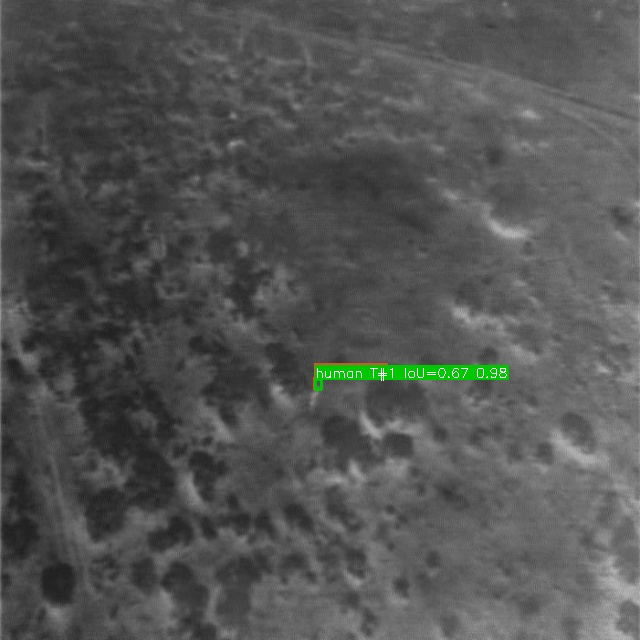
\includegraphics[width=\textwidth]{figures/birdsai_0000000361_frame0000.jpg}%
    \end{minipage}%
    \begin{minipage}[b]{0.333\textwidth}%
        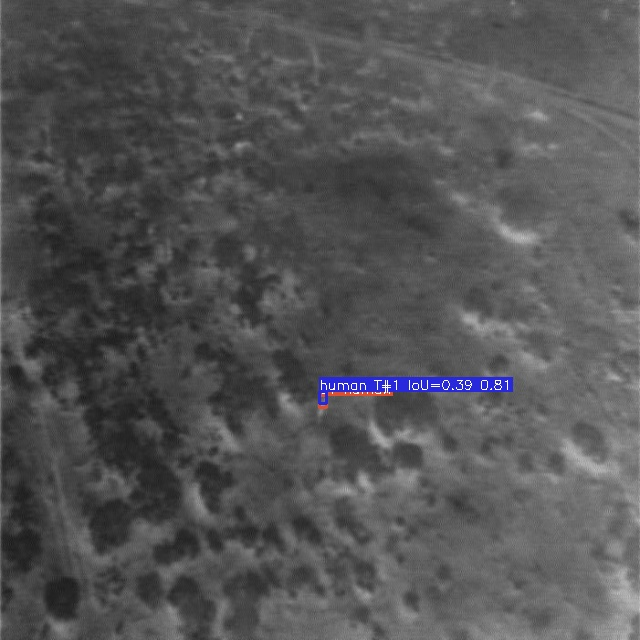
\includegraphics[width=\textwidth]{figures/birdsai_0000000361_frame0005.jpg}%
    \end{minipage}%
    \begin{minipage}[b]{0.333\textwidth}%
        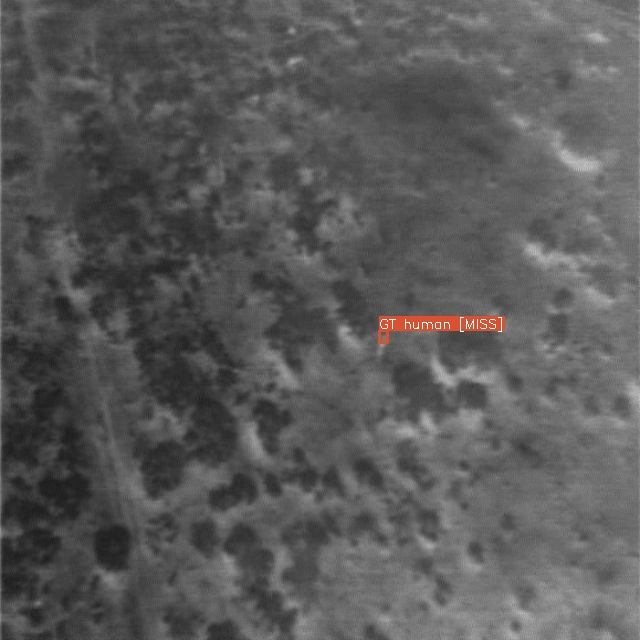
\includegraphics[width=\textwidth]{figures/birdsai_0000000361_frame0015.jpg}%
    \end{minipage}
    \caption{SAM2 SOT results on BIRDSAI sequence \texttt{0000000361} (human category): frame 0, 5, and 15.
             Bounding box colours: \textcolor{orange}{orange} = ground-truth box;
             \textcolor{green!70!black}{green} = predicted box with IoU $\geq 0.5$ (true positive);
             \textcolor{blue}{blue} = predicted box with IoU $< 0.5$ (false positive).}
    \label{fig:sam2_birdsai_animal}
\end{figure}

Figure~\ref{fig:sam2_birdsai_animal2} shows a different human sequence in which the target is noticeably larger and exhibits a stronger thermal signature, appearing as a brighter blob in the infrared imagery.
As a result, SAM2 achieves near-complete tracking throughout the sequence with no observable track loss.
However, localisation is not always precise: in several frames the predicted bounding box is slightly misaligned with the ground truth, falling below the IoU threshold and being counted as a false positive.
More critically, the bottom-right frame illustrates a failure mode that arises when the target moves through a crowd: surrounded by other individuals with similar thermal appearances, SAM2's mask propagation drifts onto a neighbouring person, assigning the predicted box to the wrong identity.
This highlights a fundamental limitation of prompt-based tracking in scenes with multiple similar-looking targets in close proximity.

\begin{figure}[htbp]
    \centering
    \begin{minipage}[b]{0.333\textwidth}%
        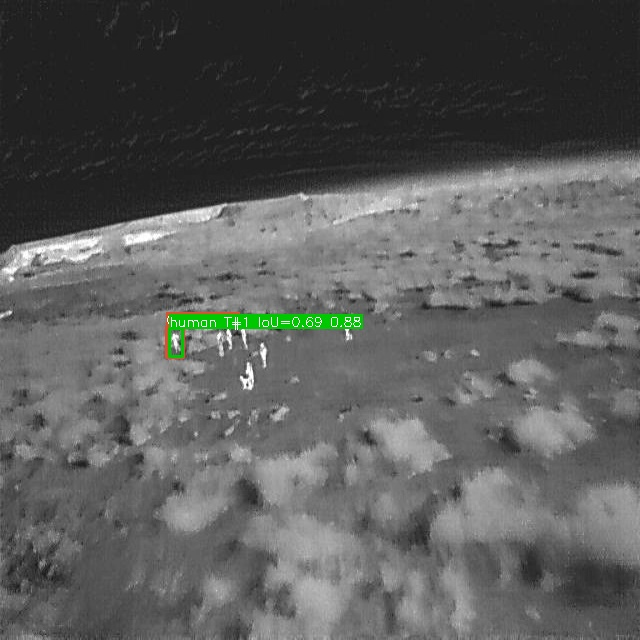
\includegraphics[width=\textwidth]{figures/birdsai_0000000371_s1_frame0000.jpg}%
    \end{minipage}%
    \begin{minipage}[b]{0.333\textwidth}%
        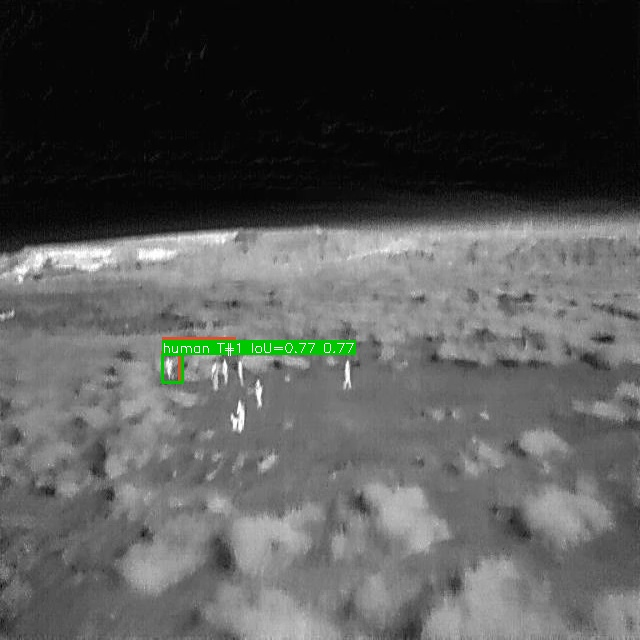
\includegraphics[width=\textwidth]{figures/birdsai_0000000371_s1_frame0010.jpg}%
    \end{minipage}%
    \begin{minipage}[b]{0.333\textwidth}%
        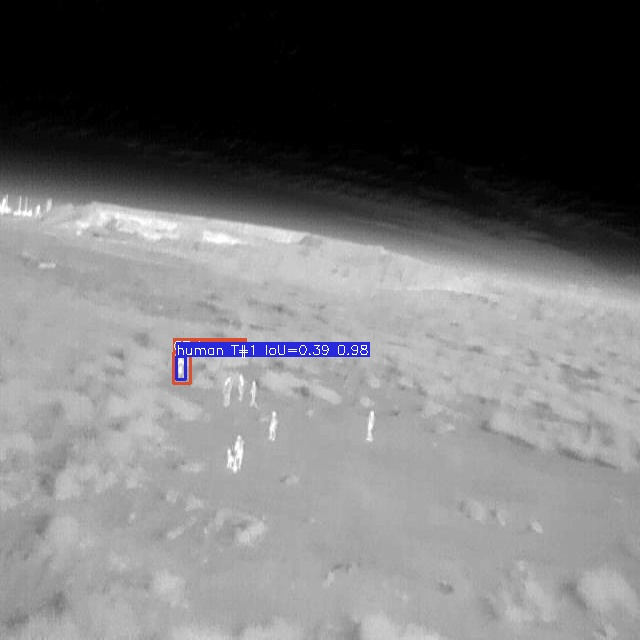
\includegraphics[width=\textwidth]{figures/birdsai_0000000371_s1_frame0040.jpg}%
    \end{minipage}%
    \\[\smallskipamount]%
    \begin{minipage}[b]{0.333\textwidth}%
        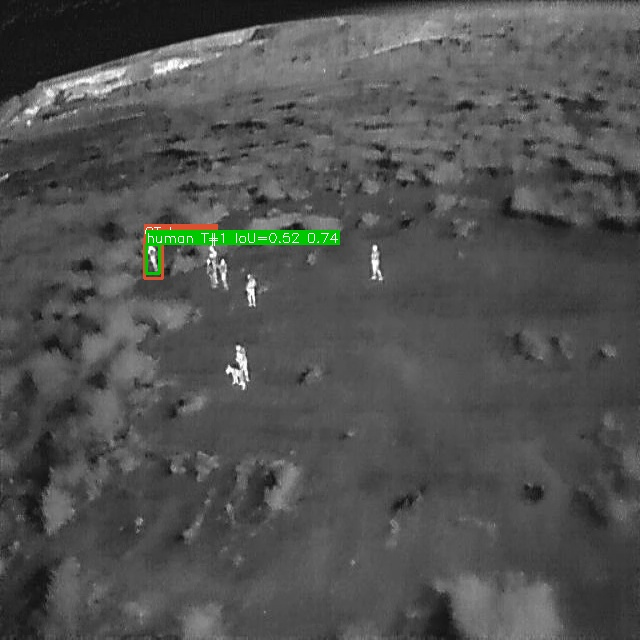
\includegraphics[width=\textwidth]{figures/birdsai_0000000371_s1_frame0151.jpg}%
    \end{minipage}%
    \begin{minipage}[b]{0.333\textwidth}%
        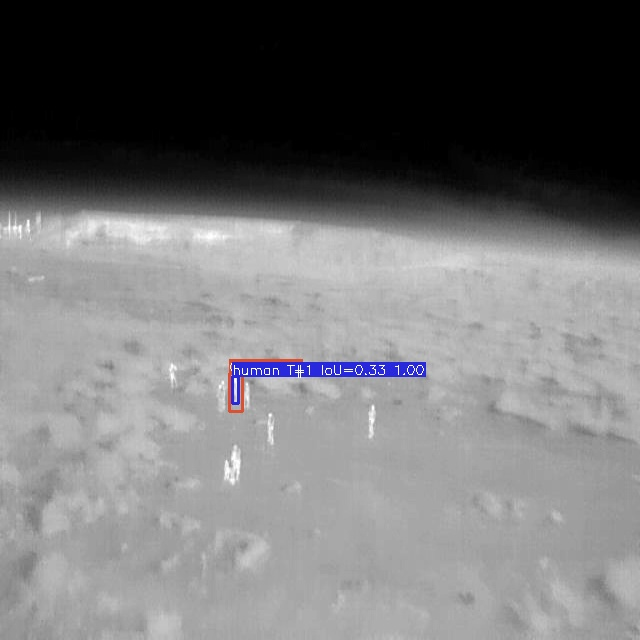
\includegraphics[width=\textwidth]{figures/birdsai_0000000371_s2_frame0050.jpg}%
    \end{minipage}%
    \begin{minipage}[b]{0.333\textwidth}%
        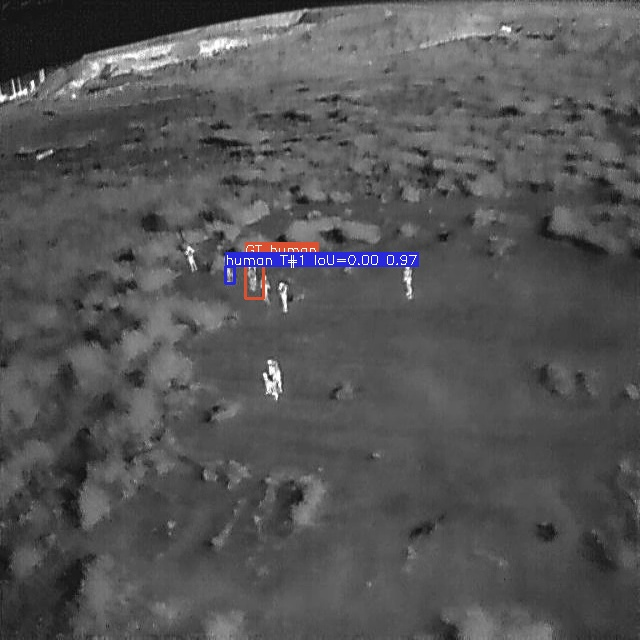
\includegraphics[width=\textwidth]{figures/birdsai_0000000371_s9_frame0232.jpg}%
    \end{minipage}
    \caption{SAM2 SOT results on BIRDSAI sequence \texttt{0000000371} (human category).
             Top row: sequence 1, frames 0, 10, and 40.
             Bottom row: sequence 1 frame 151, sequence 2 frame 50, and sequence 9 frame 232.
             Bounding box colours: \textcolor{orange}{orange} = ground-truth box;
             \textcolor{green!70!black}{green} = predicted box with IoU $\geq 0.5$ (true positive);
             \textcolor{blue}{blue} = predicted box with IoU $< 0.5$ (false positive).}
    \label{fig:sam2_birdsai_animal2}
\end{figure}

Figure~\ref{fig:sam2_birdsai_animal3} shows representative frames from the animal category, where targets are visibly larger than the human instances examined earlier.
Notably, SAM2's predicted bounding boxes often fit the target more tightly than the ground-truth annotations: because SAM2 produces segmentation masks that closely conform to the object boundary, the derived boxes tend to be more precise, whereas the ground-truth boxes in BIRDSAI are sometimes loosely drawn around the animal.
This annotation misalignment can paradoxically penalise SAM2 in IoU-based evaluation, as a tighter prediction around the true object extent may still fall below the 0.5 threshold when matched against an imprecise ground-truth box.

\begin{figure}[htbp]
    \centering
    \begin{minipage}[b]{0.2\textwidth}%
        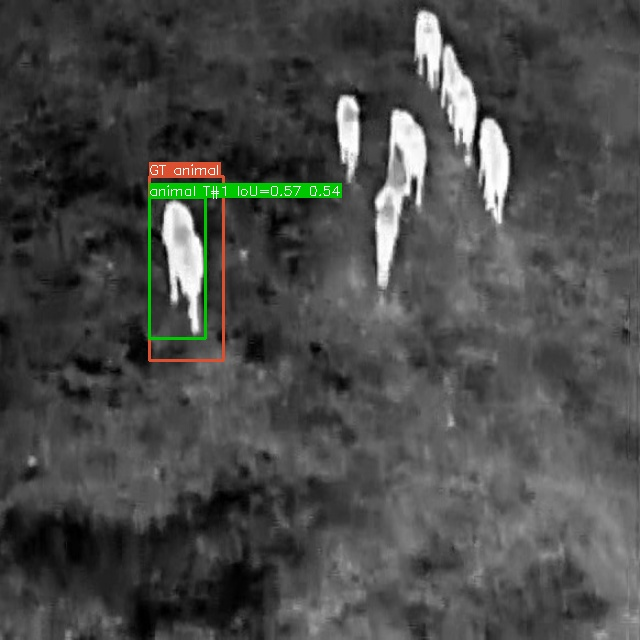
\includegraphics[width=\textwidth]{figures/birdsai_0000000352_s1a_frame0000.jpg}%
    \end{minipage}%
    \begin{minipage}[b]{0.2\textwidth}%
        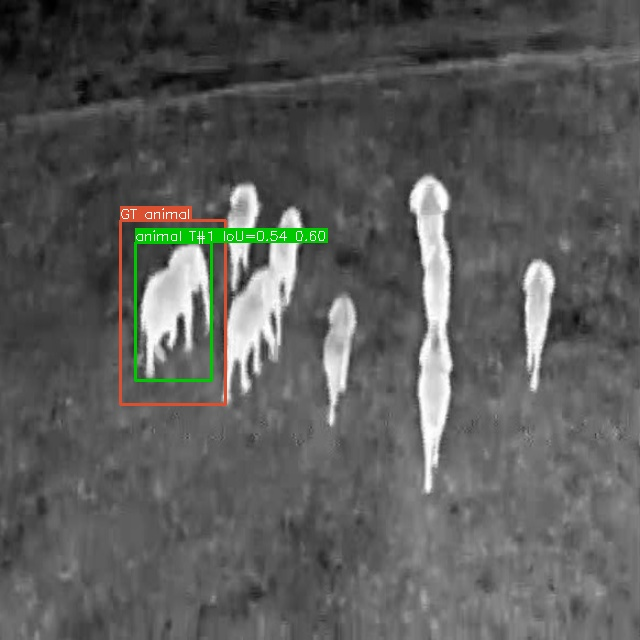
\includegraphics[width=\textwidth]{figures/birdsai_0000000352_s1b_frame0010.jpg}%
    \end{minipage}%
    \begin{minipage}[b]{0.2\textwidth}%
        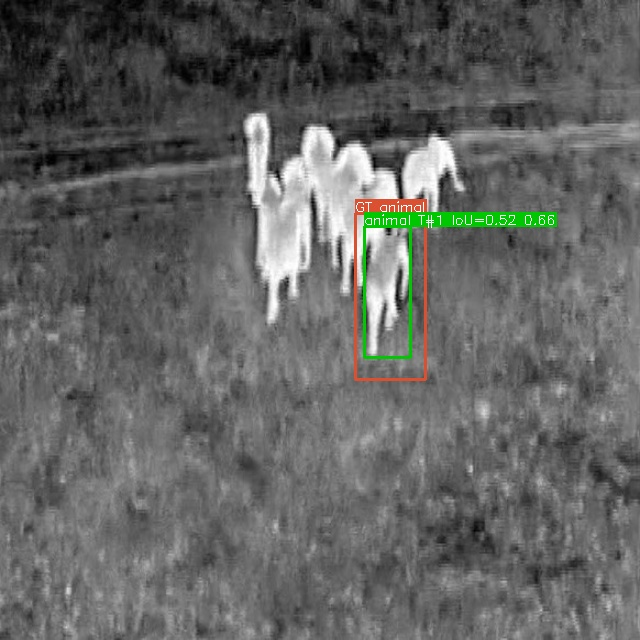
\includegraphics[width=\textwidth]{figures/birdsai_0000000352_s1c_frame0001.jpg}%
    \end{minipage}%
    \begin{minipage}[b]{0.2\textwidth}%
        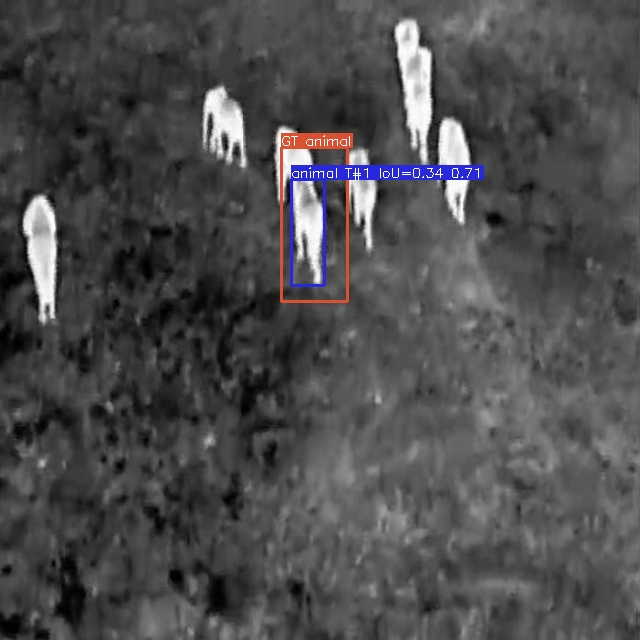
\includegraphics[width=\textwidth]{figures/birdsai_0000000352_s2a_frame0037.jpg}%
    \end{minipage}%
    \begin{minipage}[b]{0.2\textwidth}%
        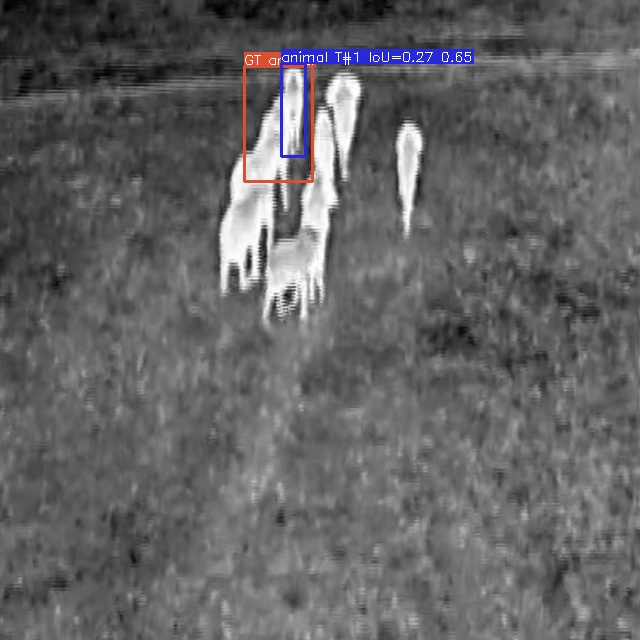
\includegraphics[width=\textwidth]{figures/birdsai_0000000352_s2b_frame0034.jpg}%
    \end{minipage}
    \caption{SAM2 SOT results on BIRDSAI sequence \texttt{0000000352} (animal category), five representative frames.
             \textcolor{orange}{Orange} = ground-truth; \textcolor{green!70!black}{green} = true positive (IoU $\geq 0.5$); \textcolor{blue}{blue} = false positive (IoU $< 0.5$).}
    \label{fig:sam2_birdsai_animal3}
\end{figure}

SAM2 also demonstrates robust tracking on smaller animal targets. As illustrated in Figure~\ref{fig:sam2_birdsai_animal4}, even under challenging 
imaging conditions — where the Air Shepherd aerial platform introduces camera shake and the target animal appears blurred or indistinct in several 
frames — SAM2 maintains stable detection and tracking throughout the sequence.

\begin{figure}[htbp]
    \centering
    \begin{minipage}[b]{0.333\textwidth}%
        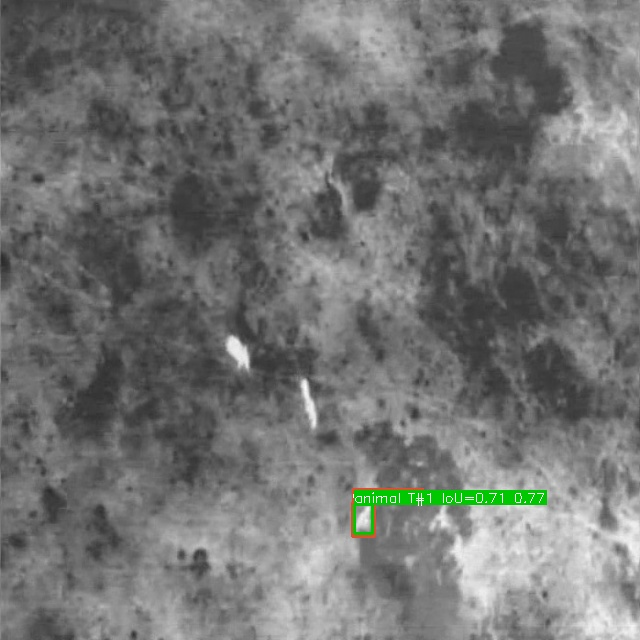
\includegraphics[width=\textwidth]{figures/birdsai_0000000058_s1_frame0000.jpg}%
    \end{minipage}%
    \begin{minipage}[b]{0.333\textwidth}%
        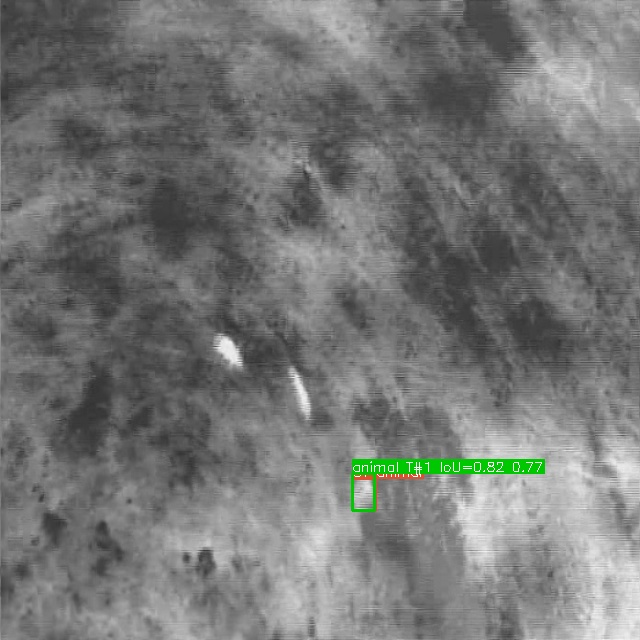
\includegraphics[width=\textwidth]{figures/birdsai_0000000058_s1_frame0009.jpg}%
    \end{minipage}%
    \begin{minipage}[b]{0.333\textwidth}%
        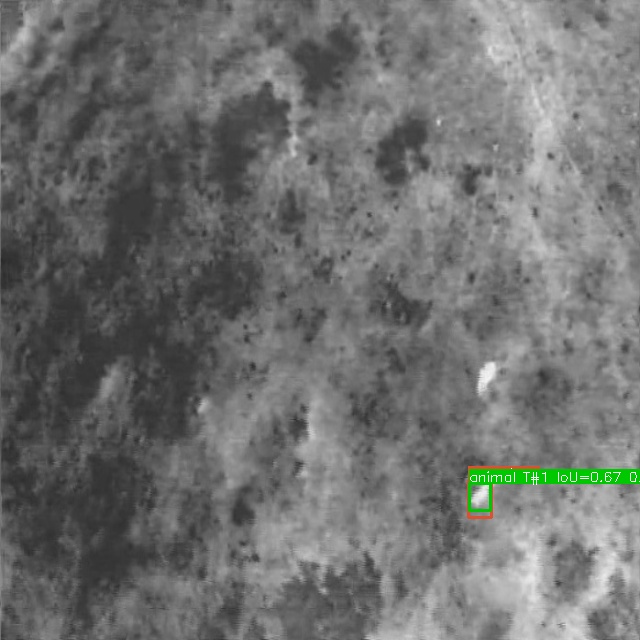
\includegraphics[width=\textwidth]{figures/birdsai_0000000058_s2_frame0004.jpg}%
    \end{minipage}
    \caption{SAM2 SOT results on BIRDSAI sequence \texttt{0000000058} (animal category), three representative frames.
             \textcolor{orange}{Orange} = ground-truth; \textcolor{green!70!black}{green} = true positive (IoU $\geq 0.5$); \textcolor{blue}{blue} = false positive (IoU $< 0.5$).}
    \label{fig:sam2_birdsai_animal4}
\end{figure}

\paragraph{OOTB.}
\paragraph{Quantitative Results}

Table~\ref{tab:sot-ootb} presents the per-category and per-size SOT results for SAM2 on the OOTB test set.

The \textit{ship} category stands out with the best performance by a large margin (Success AUC = 0.5801, Precision@20 = 0.8538, Mean IoU = 0.5805). 
This is attributable to the relatively simple and homogeneous background — open sea or sea with bridges — which makes it straightforward 
for SAM2's mask propagation to distinguish the target from the surroundings. 
You can find an example in the third figure from left to right in Figure~\ref{fig:sam2_ootb}.

In contrast, the \textit{train} category yields near-zero metrics across the board (Success AUC = 0.0476, Precision@20 = 0.0000), 
indicating that SAM2 fails to segment the train from the background from the very first frame (see Figure~\ref{fig:sam2_ootb}, rightmost panel), 
likely due to the elongated shape and ambiguous boundaries of trains in overhead imagery, which do not align well with SAM2's segmentation priors.

% ===== SOT Results on OOTB =====
\begin{table}[htbp]
\centering
\begin{tabular}{l cccc cc}
\toprule
\textbf{Metric} & \multicolumn{4}{c}{\textbf{Per Category}} & \multicolumn{2}{c}{\textbf{Per Size}} \\
\cmidrule(lr){2-5} \cmidrule(lr){6-7}
 & Car & Plane & Ship & Train & Small & Large \\
\midrule
N Frames      & 1\,728 & 480    & 800    & 192   & 2\,720 & 480    \\
Success AUC   & 0.2431 & 0.2047 & \textbf{0.5801} & 0.0476 & \textbf{0.3308} & 0.1909 \\
Precision@20  & 0.4074 & 0.4688 & \textbf{0.8538} & 0.0000 & \textbf{0.5184} & 0.4208 \\
Mean IoU      & 0.2157 & 0.1761 & \textbf{0.5805} & 0.0000 & \textbf{0.3106} & 0.1603 \\
\bottomrule
\end{tabular}
\caption{SAM2 SOT results on the OOTB test set (first-frame prompt). The dataset contains four object categories: \textit{Car}, \textit{Plane}, \textit{Ship}, and \textit{Train}. Objects are classified as small if their bounding box area is smaller than $32\times32$ pixels, and as large otherwise.}
\label{tab:sot-ootb}
\end{table}

The \textit{car} and \textit{plane} categories fall in between (Success AUC of 0.2431 and 0.2047 respectively), 
as they are set against more complex backgrounds — urban roads, parking lots, and runways — where SAM2 occasionally loses the target 
amid visual clutter (see Figure~\ref{fig:sam2_ootb}, two leftmost panels). 
We additionally note that the ground-truth annotations in OOTB are sometimes loosely fitted around objects, 
whereas SAM2's predicted masks can be tighter and more precise; this annotation misalignment penalises SAM2 during IoU-based evaluation, 
contributing to lower reported scores than the visual tracking quality would suggest.

\paragraph{Per-size effects on OOTB.}
A counterintuitive finding on OOTB is that small objects outperform large ones across all metrics (Success AUC: 0.3308 vs.\ 0.1909; Precision@20: 0.5184 vs.\ 0.4208). This reversal — opposite to the BIRDSAI trend — is driven by the \textit{train} category: trains are the largest objects in the dataset, yet SAM2 completely fails to track them. Because the large-size subset is dominated by these failed train sequences, the aggregate large-object metrics are severely depressed. Excluding trains, larger objects would likely follow the expected pattern of higher overlap scores.



\paragraph{Qualitative Results}\label{SOT_Qualitative}

As illustrated in Figure~\ref{fig:sam2_car16}, SAM2 successfully tracks the target car from frame 0 through frame 163. 
However, as the car begins to pass under a bridge, the visible portion of the vehicle progressively decreases. 
Consequently, SAM2's predicted bounding boxes shrink accordingly, causing the IoU with the ground-truth annotations to fall below 
the detection threshold and the corresponding frames to be classified as false negatives. 
The car becomes entirely occluded beneath the bridge in subsequent frames, during which SAM2 loses the target completely, 
resulting in missed detections. Even after the car re-emerges on the other side of the bridge (frame 218), SAM2 fails to recover tracking. 
This is a direct consequence of SAM2's clip-based propagation mechanism: predictions from each clip are used as prompts for the next, 
meaning that once the target is lost under occlusion, no valid prompt is available to re-initialise tracking. 
Notably, if a manual prompt were provided at the moment of re-appearance, SAM2 would be capable of resuming accurate tracking for all subsequent frames.
\begin{figure}[htbp]
    \centering
    \begin{minipage}[b]{0.2\textwidth}%
        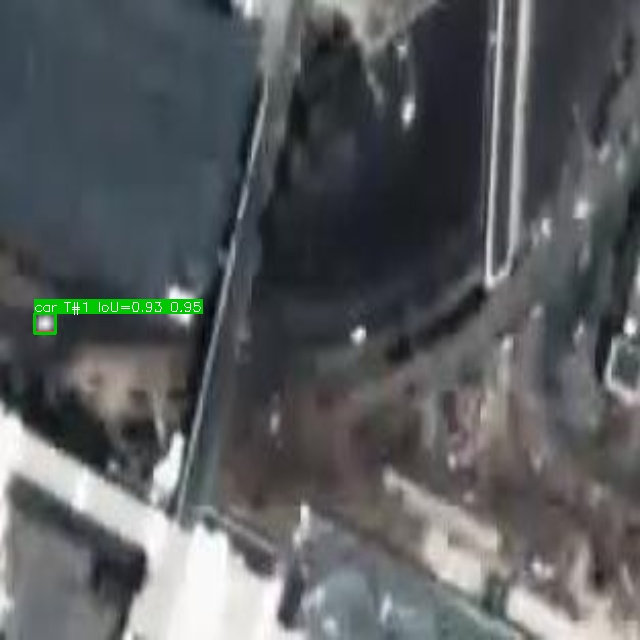
\includegraphics[width=\textwidth]{figures/car_16_frame0000.jpg}%
    \end{minipage}%
    \begin{minipage}[b]{0.2\textwidth}%
        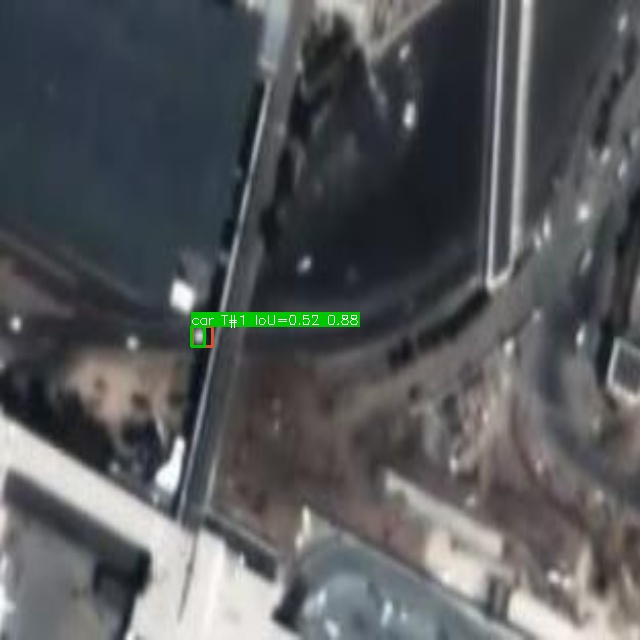
\includegraphics[width=\textwidth]{figures/car_16_frame0163.jpg}%
    \end{minipage}%
    \begin{minipage}[b]{0.2\textwidth}%
        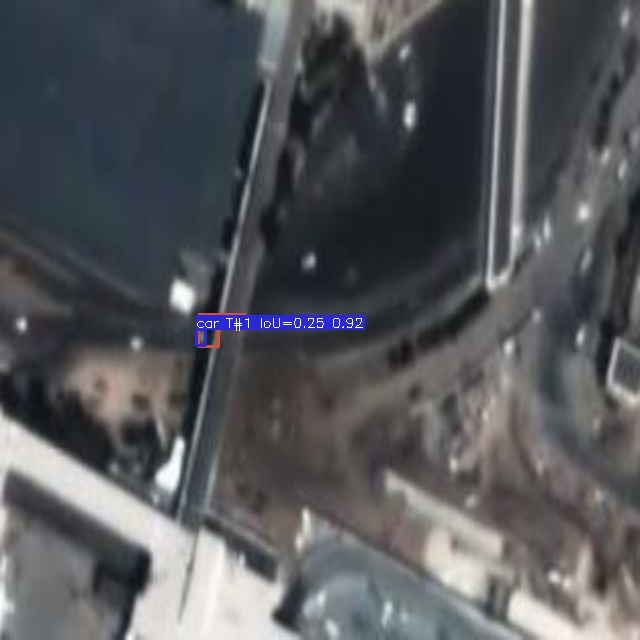
\includegraphics[width=\textwidth]{figures/car_16_frame0168.jpg}%
    \end{minipage}%
    \begin{minipage}[b]{0.2\textwidth}%
        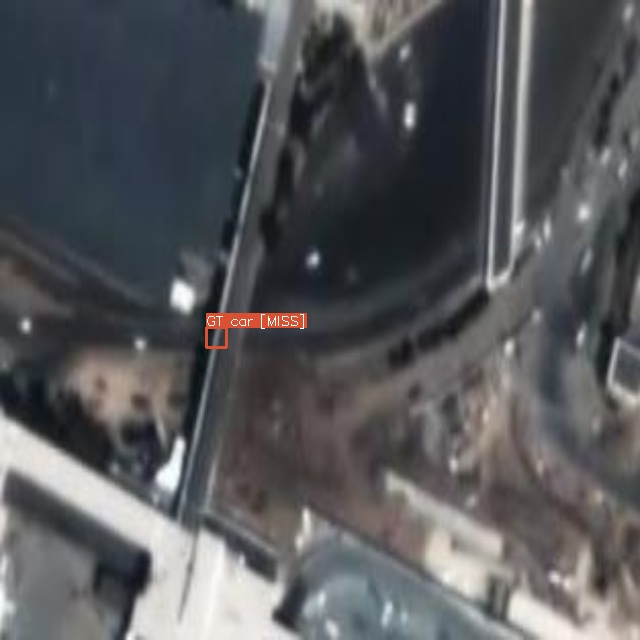
\includegraphics[width=\textwidth]{figures/car_16_frame0172.jpg}%
    \end{minipage}%
    \begin{minipage}[b]{0.2\textwidth}%
        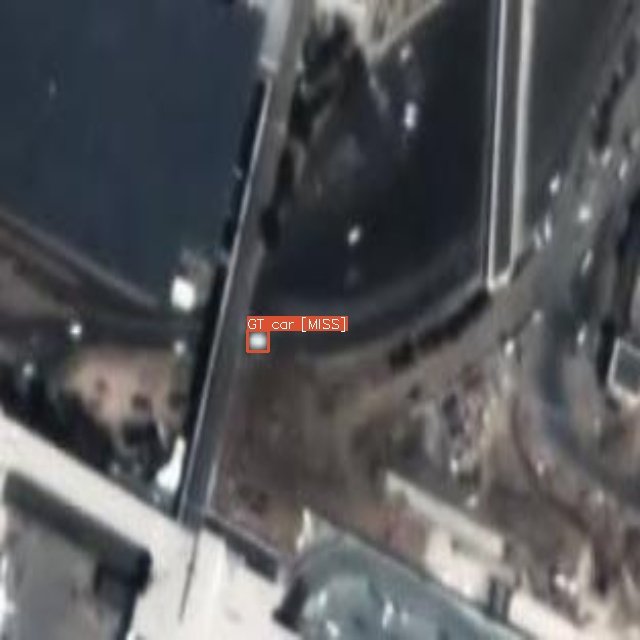
\includegraphics[width=\textwidth]{figures/car_16_frame0218.jpg}%
    \end{minipage}
    \caption{SAM2 SOT results on sequence \texttt{car\_16}: frame 0, 163, 168, 172, and 218.
             Bounding box colours: \textcolor{orange}{orange} = ground-truth box (shown as miss when no prediction is matched);
             \textcolor{green!70!black}{green} = predicted box with IoU $\geq 0.5$ (true positive);
             \textcolor{blue}{blue} = predicted box with IoU $< 0.5$ (false positive);
             \textcolor{gray}{grey} = unmatched prediction (ignored in SOT evaluation).}
    \label{fig:sam2_car16}
\end{figure}

As shown in Figure~\ref{fig:sam2_car22}, tracking failures also arise when the target is extremely small and visually indistinguishable from surrounding objects of the same class. 
In spaceborne imagery, individual cars are reduced to near-featureless bright spots, making them virtually identical in appearance to neighbouring vehicles. 
Under these conditions, SAM2's mask propagation loses discriminative power: the model cannot reliably distinguish the target instance from other cars in the scene, 
leading it to drift onto a neighbouring vehicle or lose the target entirely, resulting in missed detections. 
\begin{figure}[htbp]
    \centering
    \begin{minipage}[b]{0.2\textwidth}%
        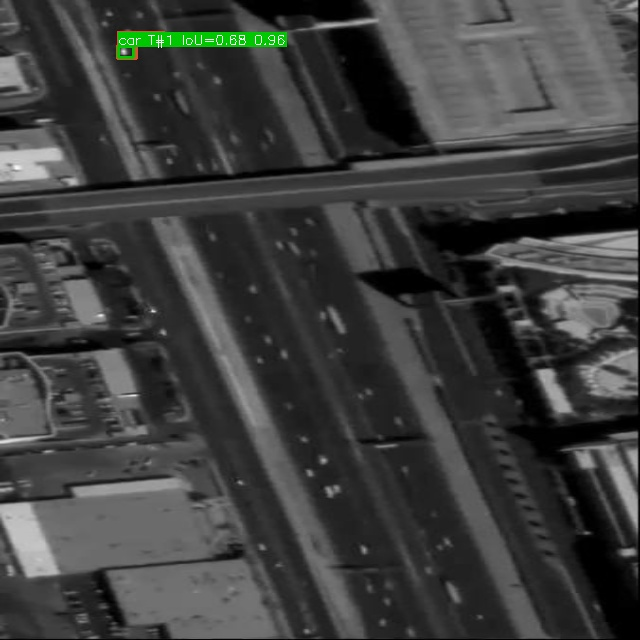
\includegraphics[width=\textwidth]{figures/car_22_frame0000.jpg}%
    \end{minipage}%
    \begin{minipage}[b]{0.2\textwidth}%
        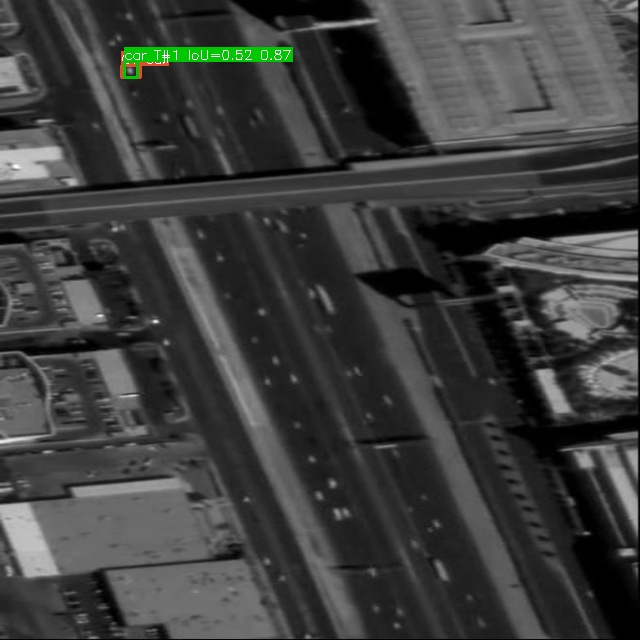
\includegraphics[width=\textwidth]{figures/car_22_frame0021.jpg}%
    \end{minipage}%
    \begin{minipage}[b]{0.2\textwidth}%
        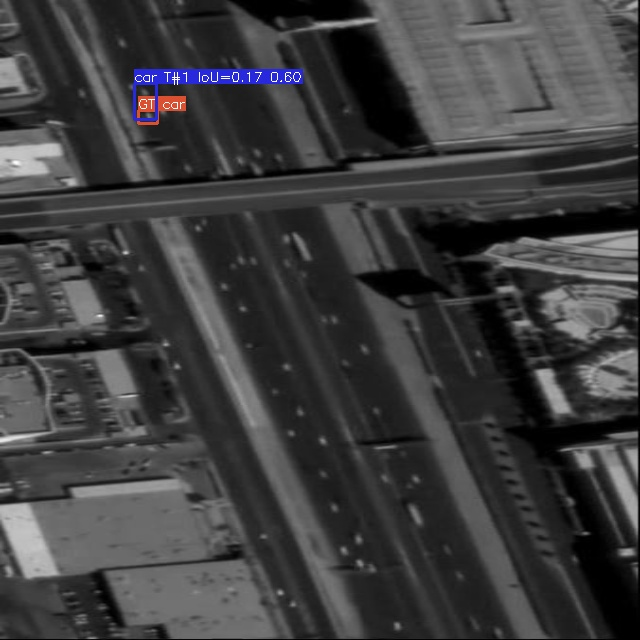
\includegraphics[width=\textwidth]{figures/car_22_frame0072.jpg}%
    \end{minipage}%
    \begin{minipage}[b]{0.2\textwidth}%
        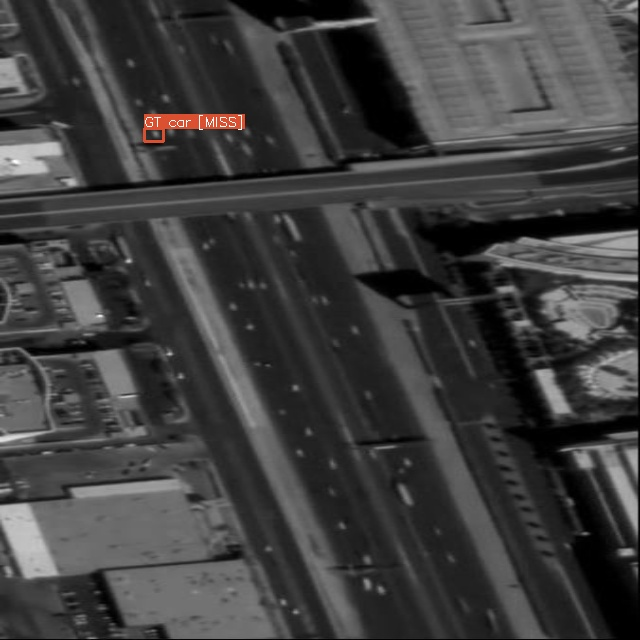
\includegraphics[width=\textwidth]{figures/car_22_frame0091.jpg}%
    \end{minipage}%
    \begin{minipage}[b]{0.2\textwidth}%
        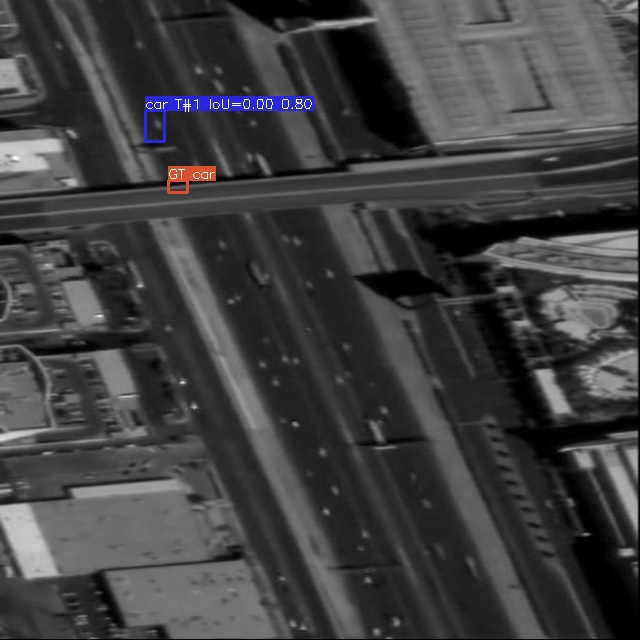
\includegraphics[width=\textwidth]{figures/car_22_frame0149.jpg}%
    \end{minipage}
    \caption{SAM2 SOT results on sequence \texttt{car\_22}: frame 0, 21, 72, 91, and 149.
             Bounding box colours: \textcolor{orange}{orange} = ground-truth box (shown as miss when no prediction is matched);
             \textcolor{green!70!black}{green} = predicted box with IoU $\geq 0.5$ (true positive);
             \textcolor{blue}{blue} = predicted box with IoU $< 0.5$ (false positive);
             \textcolor{gray}{grey} = unmatched prediction (ignored in SOT evaluation).}
    \label{fig:sam2_car22}
\end{figure}

As illustrated in Figure~\ref{fig:sam2_plane12}, SAM2 derives its predicted bounding boxes directly from the underlying segmentation mask, 
which causes them to conform tightly to the object boundary. In several frames, the predicted box is in fact a closer fit to the actual aircraft than the ground-truth annotation itself, 
which is annotated more loosely. This further corroborates the annotation misalignment effect noted earlier: 
IoU-based metrics penalise SAM2 precisely because its predictions are more precise than the reference labels, leading to an underestimation of its true tracking quality. 
\begin{figure}[htbp]
    \centering
    \begin{minipage}[b]{0.333\textwidth}%
        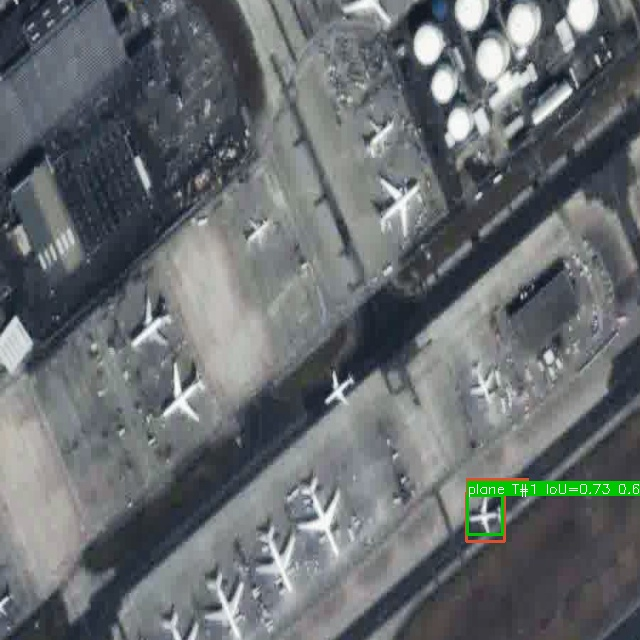
\includegraphics[width=\textwidth]{figures/plane_12_frame0000.jpg}%
    \end{minipage}%
    \begin{minipage}[b]{0.333\textwidth}%
        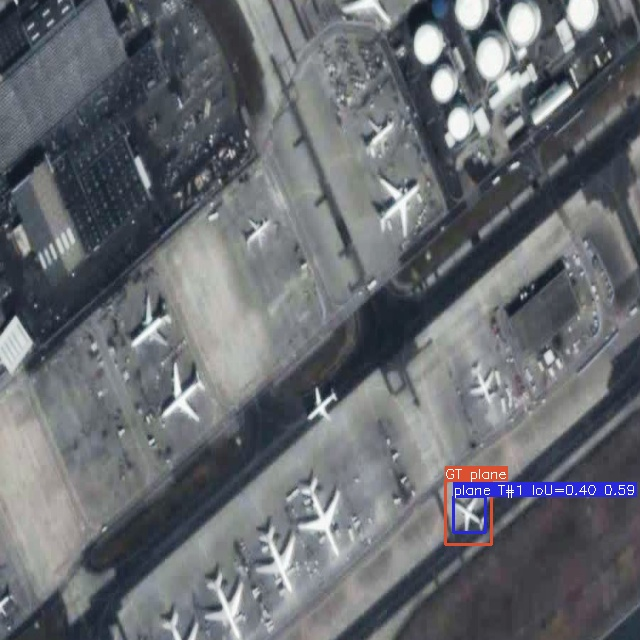
\includegraphics[width=\textwidth]{figures/plane_12_frame0035.jpg}%
    \end{minipage}%
    \begin{minipage}[b]{0.333\textwidth}%
        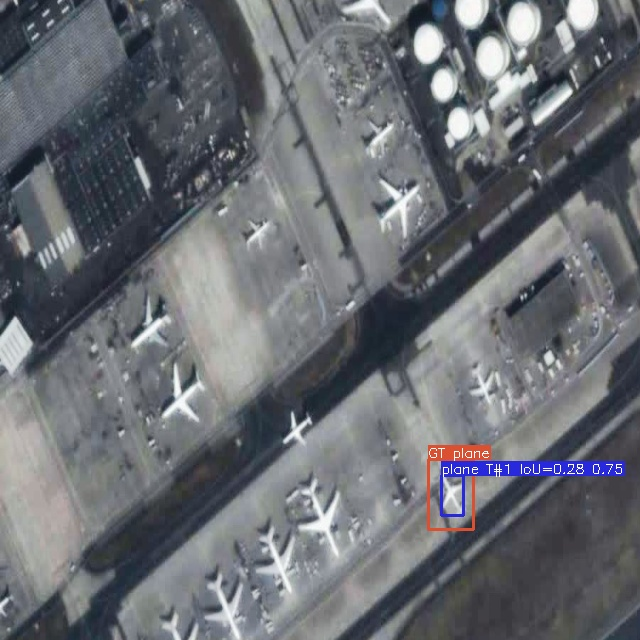
\includegraphics[width=\textwidth]{figures/plane_12_frame0083.jpg}%
    \end{minipage}
    \caption{SAM2 SOT results on sequence \texttt{plane\_12}: frame 0, 35, and 83.
             Bounding box colours: \textcolor{orange}{orange} = ground-truth box (shown as miss when no prediction is matched);
             \textcolor{green!70!black}{green} = predicted box with IoU $\geq 0.5$ (true positive);
             \textcolor{blue}{blue} = predicted box with IoU $< 0.5$ (false positive);
             \textcolor{gray}{grey} = unmatched prediction (ignored in SOT evaluation).}
    \label{fig:sam2_plane12}
\end{figure}

\begin{figure}[htbp]
    \centering
    \begin{minipage}[b]{0.25\textwidth}%
        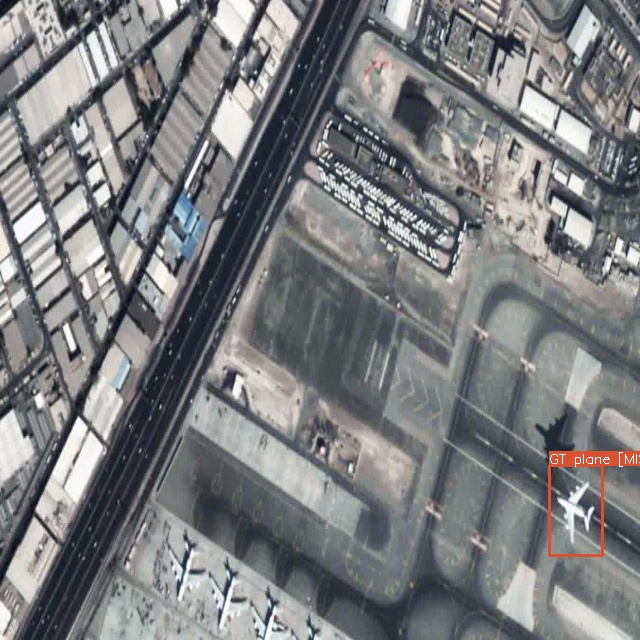
\includegraphics[width=\textwidth]{figures/plane_21_frame0000.jpg}%
    \end{minipage}%
    \begin{minipage}[b]{0.25\textwidth}%
        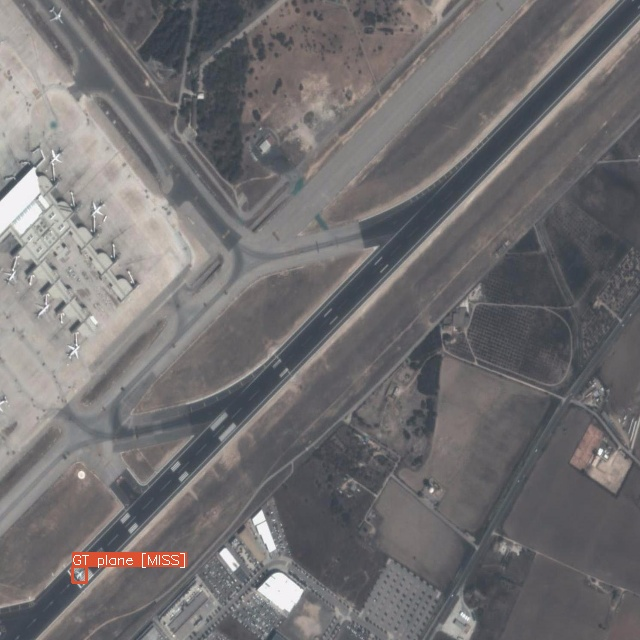
\includegraphics[width=\textwidth]{figures/plane_25_frame0024.jpg}%
    \end{minipage}%
    \begin{minipage}[b]{0.25\textwidth}%
        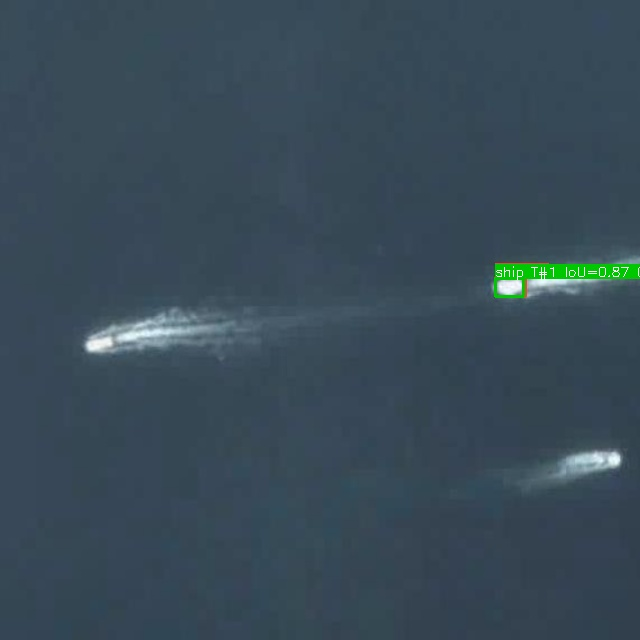
\includegraphics[width=\textwidth]{figures/ship_2_frame0000.jpg}%
    \end{minipage}%
    \begin{minipage}[b]{0.25\textwidth}%
        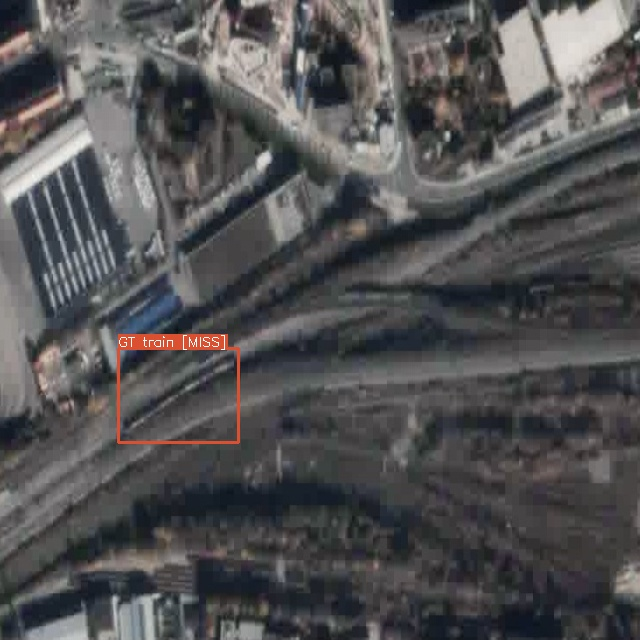
\includegraphics[width=\textwidth]{figures/train_2_frame0000.jpg}%
    \end{minipage}
    \caption{SAM2 SOT results on sequences \texttt{plane\_21} (frame 0), \texttt{plane\_25} (frame 24), \texttt{ship\_2} (frame 0), and \texttt{train\_2} (frame 0).
             Bounding box colours: \textcolor{orange}{orange} = ground-truth box (shown as miss when no prediction is matched);
             \textcolor{green!70!black}{green} = predicted box with IoU $\geq 0.5$ (true positive);
             \textcolor{blue}{blue} = predicted box with IoU $< 0.5$ (false positive);
             \textcolor{gray}{grey} = unmatched prediction (ignored in SOT evaluation).}
    \label{fig:sam2_ootb}
\end{figure}

\hypertarget{Multi-Object Tracking (MOT)}{%
\subsubsection{Multi-Object Tracking (MOT)}\label{MOT}}

\paragraph{Quantitative Results}\label{MOT_Quantitative}
Tables~\ref{tab:mot-per-category} and~\ref{tab:mot-per-size} break down performance by object category and size, revealing consistent trends across all three models.

All models perform substantially better on large objects than small ones. 
Faster R-CNN achieves the highest recall for large objects (0.7903) and a strong MOTA of 0.5826 and IDF1 of 0.8076, 
demonstrating that its region-proposal mechanism is well-suited to localising larger targets. 
YOLO11n also performs competitively on large objects, with the highest precision (0.8424) and a solid MOTA of 0.3412, 
while SAM2 lags behind in recall (0.2130) despite reasonable precision (0.6545). 
For small objects, all models struggle considerably: Faster R-CNN achieves the best recall (0.4769) but at the cost of an extremely high false-positive rate, 
yielding a MOTA of $-2.8237$. YOLO11n and SAM2 are more conservative, with recalls of only 0.0812 and 0.2143 respectively, 
though SAM2 achieves the best IDF1 among the three for small objects (0.2368), suggesting more consistent track identity despite low detection coverage.

These size-based trends directly explain the per-category results. 
Since humans in the BIRDSAI dataset are generally small targets, all models exhibit substantially weaker performance on the human category. 
YOLO11n is the most extreme case: it achieves near-perfect precision on humans (0.9830) but an extremely low recall of 0.0517, 
indicating that it rarely detects humans at all, and those it does detect are highly confident true positives. 
Faster R-CNN recovers the most human detections (recall 0.5622, IDF1 0.4965), though still with a negative MOTA ($-0.1907$) due to identity switches. 
SAM2 performs poorly on both metrics for humans (recall 0.1180, IDF1 0.1369), 
as its prompt-and-propagate approach is particularly sensitive to the small apparent size and low contrast of human targets in thermal imagery.
For the animal category, where targets are more varied in size but generally larger than humans, 
all models improve noticeably. YOLO11n achieves the best animal precision (0.6864) and IDF1 (0.5009), 
while Faster R-CNN leads in recall (0.7032). SAM2 shows moderate animal performance (MOTA 0.0424, IDF1 0.3366), 
benefiting from the larger and more stable appearance of animal targets compared to humans.

It is also worth noting that the BIRDSAI dataset exhibits a significant class imbalance between categories: 
animal instances substantially outnumber human instances (num\_gt: 55\,101 vs.\ 16\,804), 
which may bias detection models such as Faster R-CNN and YOLO11n towards predicting the animal class, 
further contributing to the low recall observed for humans. 
To address this imbalance, future work will explore training with a weighted cross-entropy loss 
or other class-balancing strategies to improve human detection performance.
% ----- Per-category table (merged) -----
\begin{table}[htbp]
\centering
\begin{tabular}{l ccc ccc}
\toprule
\textbf{Metric} & \multicolumn{3}{c}{\textbf{Animal}} & \multicolumn{3}{c}{\textbf{Human}} \\
\cmidrule(lr){2-4} \cmidrule(lr){5-7}
 & SAM2 & FRCNN & YOLO & SAM2 & FRCNN & YOLO \\
\midrule
TP        & 13\,181          & \textbf{38\,749} & 21\,728          & 1\,977           & \textbf{9\,448}  & 869     \\
FP        & \textbf{10\,880} & 84\,739          & 9\,929           & 10\,154          & 11\,805          & \textbf{15} \\
FN        & 41\,079          & \textbf{16\,352} & 33\,373          & 14\,774          & \textbf{7\,356}  & 15\,935 \\
Num GT    & 54\,260          & 55\,101          & 55\,101          & 16\,751          & 16\,804          & 16\,804 \\
Precision & 0.5478           & 0.3138           & \textbf{0.6864}  & 0.1630           & 0.4445           & \textbf{0.9830} \\
Recall    & 0.2429           & \textbf{0.7032}  & 0.3943           & 0.1180           & \textbf{0.5622}  & 0.0517  \\
MOTA      & 0.0424           & $-0.8838$        & \textbf{0.1832}  & $-0.4881$        & $-0.1907$        & \textbf{0.0314} \\
IDF1      & 0.3366           & 0.4339           & \textbf{0.5009}  & 0.1369           & \textbf{0.4965}  & 0.0983  \\
ID Sw.    & \textbf{0}       & 2\,708           & 1\,705           & \textbf{0}       & 847              & 327     \\
\bottomrule
\end{tabular}
\caption{Per-category MOT results on the BIRDSAI test set.}
\label{tab:mot-per-category}
\end{table}

% ----- Per-size table (merged) -----
\begin{table}[htbp]
\centering
\begin{tabular}{l ccc ccc}
\toprule
\textbf{Metric} & \multicolumn{3}{c}{\textbf{Small}} & \multicolumn{3}{c}{\textbf{Large}} \\
\cmidrule(lr){2-4} \cmidrule(lr){5-7}
 & SAM2 & FRCNN & YOLO & SAM2 & FRCNN & YOLO \\
\midrule
TP        & 5\,789           & \textbf{13\,131} & 2\,236           & 9\,369           & \textbf{35\,066} & 20\,361 \\
FP        & 16\,089          & 89\,145          & \textbf{6\,136}  & \textbf{4\,945}  & 7\,399           & 3\,808  \\
FN        & 21\,230          & \textbf{14\,404} & 25\,299          & 34\,623          & \textbf{9\,304}  & 24\,009 \\
Num GT    & 27\,019          & 27\,535          & 27\,535          & 43\,992          & 44\,370          & 44\,370 \\
Precision & 0.2646           & 0.1284           & \textbf{0.2671}  & 0.6545           & 0.8258           & \textbf{0.8424} \\
Recall    & 0.2143           & \textbf{0.4769}  & 0.0812           & 0.2130           & \textbf{0.7903}  & 0.4589  \\
MOTA      & $-0.3812$        & $-2.8237$        & \textbf{$-0.1641$} & 0.1006         & \textbf{0.5826}  & 0.3412  \\
IDF1      & \textbf{0.2368}  & 0.2023           & 0.1245           & 0.3214           & \textbf{0.8076}  & 0.5941  \\
ID Sw.    & \textbf{0}       & 1\,737           & 618              & \textbf{0}       & 1\,818           & 1\,414  \\
\bottomrule
\end{tabular}
\caption{Per-size MOT results on the BIRDSAI test set.}
\label{tab:mot-per-size}
\end{table}


\paragraph{Qualitative Results}\label{MOT_Qualitative}

Figure~\ref{fig:mot_birdsai_comparison} presents a qualitative comparison of all three models on the same frame, 
providing visual confirmation of the trends observed in the quantitative analysis. 
SAM2 exhibits a large number of false negatives: since it can only track objects visible in the first frame, 
any target that enters the scene later cannot be detected, which is particularly problematic in the BIRDSAI dataset 
where new animals and humans frequently appear throughout the video sequence. 
Faster R-CNN, consistent with its high recall but low precision, produces numerous false positive detections, 
annotating regions that contain no actual targets. YOLO11n takes a more conservative approach, 
generating fewer but more confident predictions; however, it also misses a considerable number of targets, 
and one identity switch is visible in the frame, where a tracked object has been assigned a new ID mid-sequence. 
Overall, the qualitative results align well with the quantitative findings reported in 
Tables~\ref{tab:birdsai_mot-overall} and~\ref{tab:mot-per-size}.

\begin{figure}[htbp]
    \centering
    \begin{minipage}[b]{0.333\textwidth}%
        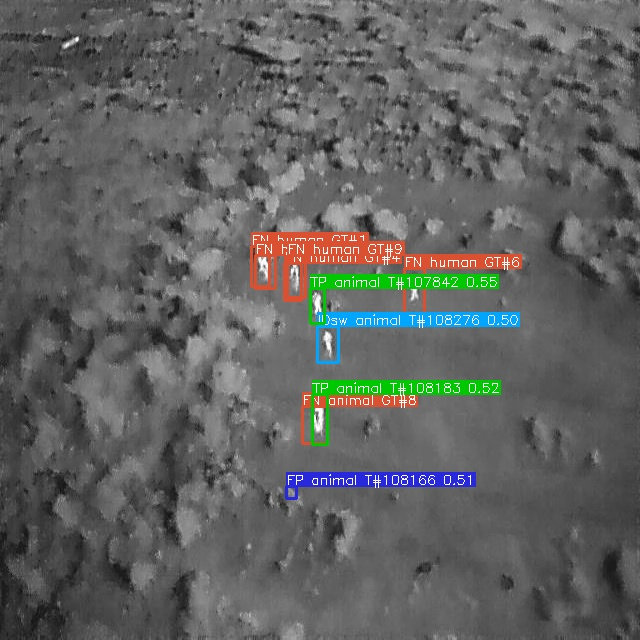
\includegraphics[width=\textwidth]{figures/mot_yolo_0000000371_frame0623.jpg}%
    \end{minipage}%
    \begin{minipage}[b]{0.333\textwidth}%
        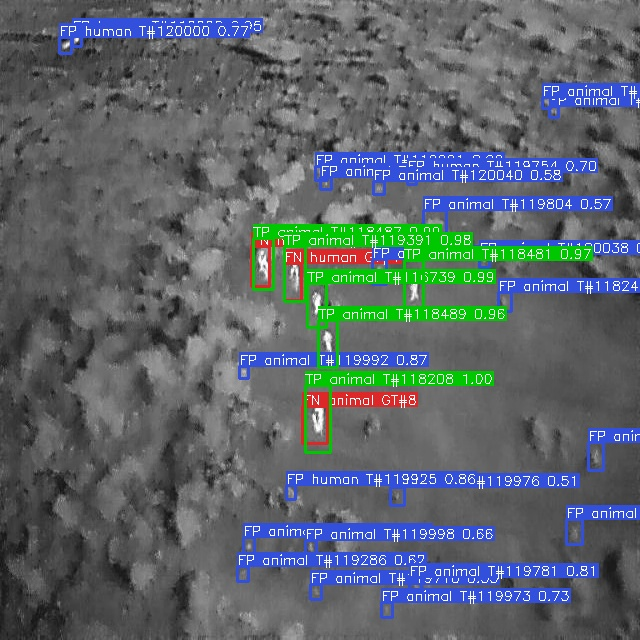
\includegraphics[width=\textwidth]{figures/mot_frcnn_0000000371_frame0623.jpg}%
    \end{minipage}%
    \begin{minipage}[b]{0.333\textwidth}%
        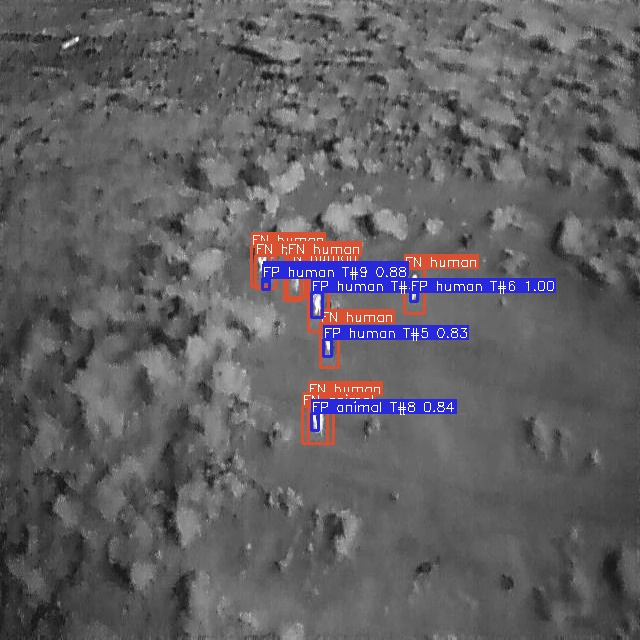
\includegraphics[width=\textwidth]{figures/mot_sam2_0000000371_frame0623.jpg}%
    \end{minipage}
    \caption{MOT results on BIRDSAI sequence \texttt{0000000371}, frame 623.
             Left: YOLO11n; centre: Faster R-CNN v2; right: SAM2.
             Bounding box colours indicate detection outcome:
             \textcolor{green}{green} = TP, \textcolor{blue}{blue} = FP, \textcolor{red}{red} = FN, \textcolor{orange}{orange} = ID switch.}
    \label{fig:mot_birdsai_comparison}
\end{figure}

\subsection{Performance by Frame per Second (FPS)}

To be updated.

\subsection{Performance by Signal to Noise Ratio (SNR)}

To be updated.

\subsection{Compliance Overview}

Table~\ref{tab:compliance-overview} provides a high-level compliance overview for each tested algorithm across all test dimensions defined in D5.
Each cell indicates whether the algorithm's performance on that dimension is \textbf{C} (Compliant), \textbf{Mi} (Minor non-compliance), or \textbf{Ma} (Major non-compliance).
Detailed results and non-compliance analyses are presented in the subsections that follow. We will complete the Table~\ref{tab:compliance-overview} in report version 2.

\begin{table}[h]
\centering
\begin{tabular}{|l|c|c|c|c|c|c|}
\hline
\multirow{2}{*}{\textbf{Algorithm}} & \multicolumn{2}{c|}{\textbf{Task}} & \multicolumn{2}{c|}{\textbf{Object Size}} & \multirow{2}{*}{\textbf{FPS}} & \multirow{2}{*}{\textbf{SNR}} \\
\cline{2-5}
 & SOT & MOT & Small & Large & & \\
\hline
SAM2 & C & Ma & C & C & -- & -- \\
\hline
YOLO & Ma & C & Mi & C & -- & -- \\
\hline
FasterRCNN & Ma & C & Mi & C & -- & -- \\
\hline
Grounding DINO & -- & -- & -- & -- & -- & -- \\
\hline
$\cdots$ & -- & -- & -- & -- & -- & -- \\
\hline
\end{tabular}
\caption{Compliance overview per algorithm and test dimension. C\,=\,Compliant; Mi\,=\,Minor non-compliance; Ma\,=\,Major non-compliance; --\,=\,Under development (to be reported in the final report).\label{tab:compliance-overview}}
\end{table}


\bibliographystyle{plain}
\bibliography{references}

\end{document}
